\chapter{Appendix: Ethernet Frame Delivery Delay Estimation}
\label{appH}

\begin{center}
	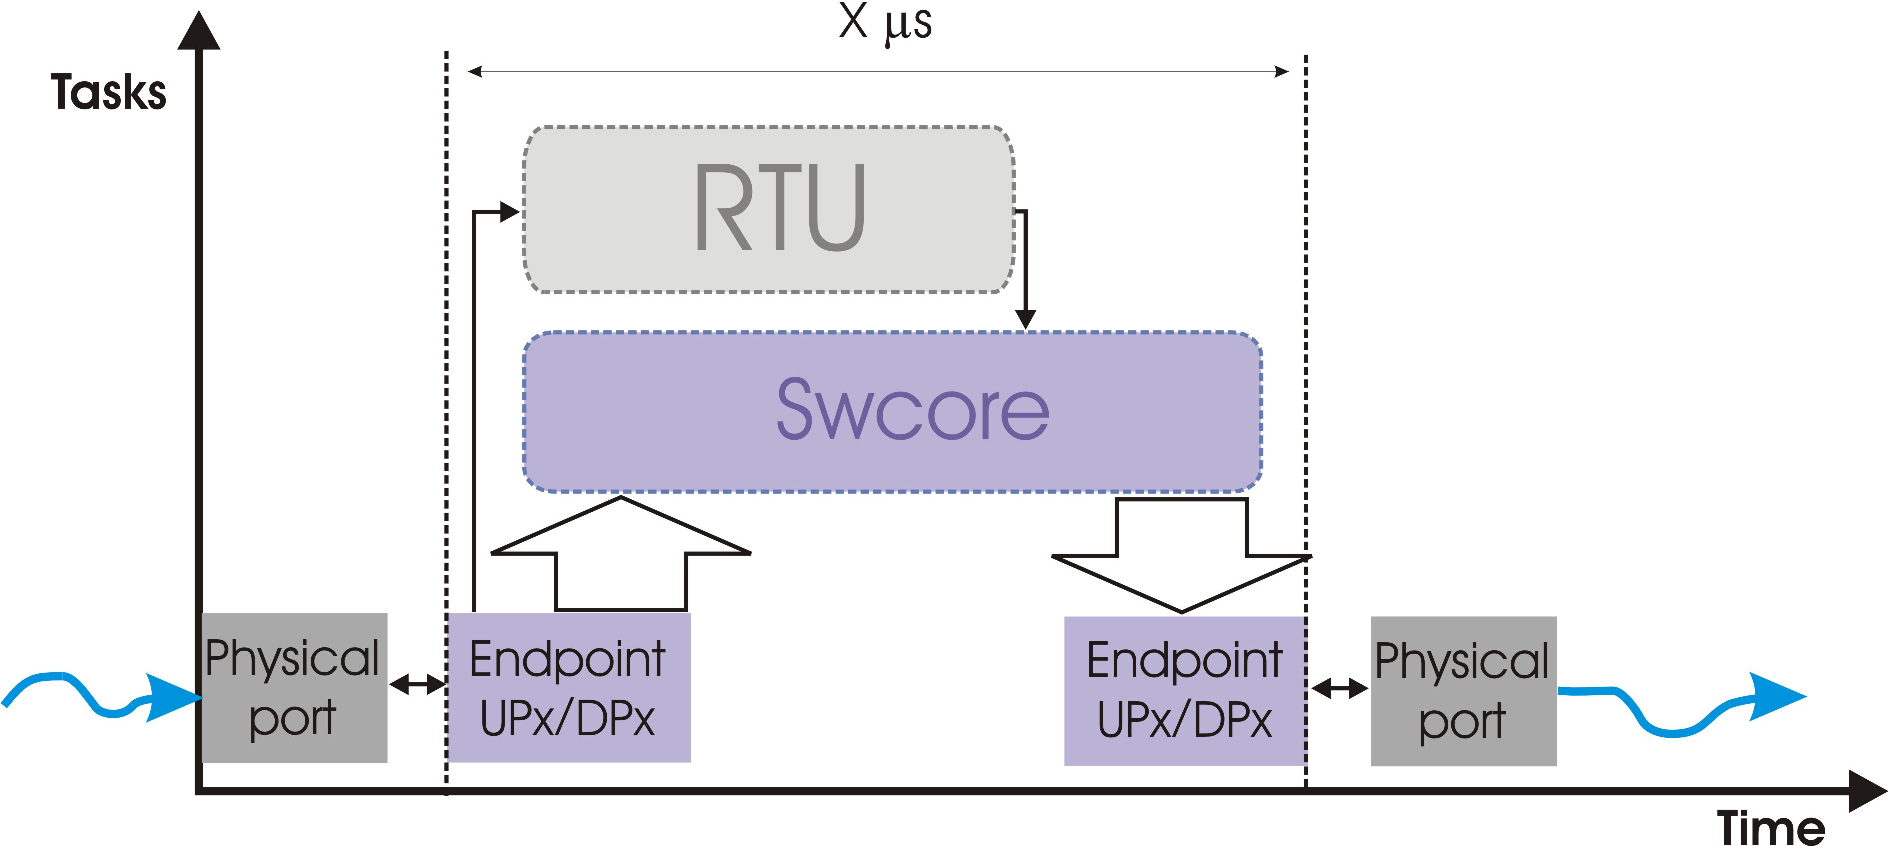
\includegraphics[scale=0.30]{../../../../figures/robustness/switchRouting.ps}
	\captionof{figure}{WR Switch routing using Swcore and RTU (not to
			  scale).}
	\label{fig:swRouting}
\end{center}

It is estimated that WR Switch routing ($delay_{sw}$) takes between
13 $\mu$s and 80 $\mu$s for highest priority traffic (size: 1500bytes), provided
no traffic congestion occurs and depending on the size of output buffer. In
order to estimate minimum Granularity Window a few more values needs to be
introduced and estimated. We define the time it takes for a WR Node to send an
Ethernet frame as Transmission Delay ($delay_{n\_tx}$) and the time it takes a
WR Node to receive Ethernet frame as Reception Delay ($delay_{n\_rx}$). The
delay introduced by physical connection (i.e. the time it takes for a frame to
travel through the physical medium) is defined as Link Delay ($delay_{f\_link}$
[$\frac{\mu s}{km}$] and $delay_{c\_link}$ [$\frac{\mu s}{km}$] for fibre and
copper respectively). Thus, the final equation to estimate the delay of single
Ethernet frame delivery time can be defined by the following equation:

\begin{equation}
	Delay_{frame} = D_{f} * delay_{f\_link} + D_{c} * delay_{c\_link} + 
	N * delay_{sw} + delay_{n\_tx} + delay_{n\_rx}
\end{equation}	    

where $D_f$ [$km$] is the total length of fibre connection and $D_f$ [$km$] is
the total length of copper connection. $N$ is the number of WR Switches on
the way.

In the following estimations, the worst case scenario of Ethernet frame size is
taken into account. It means that we always assume the size of the frame is
maximum, i.e. 1500bytes. Transmission of 1500bytes over Gigabit Ethernet takes
$~13\mu s$. 


\paragraph{Ethernet Frame Transmission Delay Estimation.} 

For simplicity, no encoding is assumed. The delay of frame transmission depends
on the remaining size of the currently sent frame and the number of packages
already enqueued in the output buffer. Assuming that sending 1500 bytes takes
$~13\mu s$, $delay_{n\_tx}= [ 0 \mu s \div (13 + B * 13)\mu s]$
where $B$ is the number of frames in the output buffer (maximum $B$ is the size
of the output buffer). 

\paragraph{Ethernet Frame Reception Delay estimation.} 

The reception of maximum size Ethernet frame is estimated to take $~13\mu s$
\footnote{The time of 1500byte Ethernet Frame reception is $12.176\mu s$,
in the calculations, it is overestimated to $13\mu s$.}  .
It is assumed that no decoding is performed. Therefore $delay_{n\_rx} = 13\mu
s$. 

\paragraph{Link Delay estimation.} 

The delay introduced by link is estimated to be 5 [$\frac{\mu s}{km}$] for fibre
\cite{PropagationDelay} (\cm{i'm not sure about the source}) and 5
[$\frac{\mu
s}{km}$] copper \cite{FAIRtiming} link.

\paragraph{Switch Routing Delay estimation.} 

The delay introduced on the switch is more complicated to estimate. The
reception delay and transmission delay overlap with the delay introduced by
storing and routing.
\begin{equation}
	delay_{sw} =  \delta + delay_{RTU} + delay_{n\_tx}  
          \; \; \; \; \;
          for 
	  \; \; \; \; \;
	  (delay_{n\_rx} - \delta) < delay_{RTU}
\end{equation}	 
\begin{equation}
	delay_{sw} =  delay_{n\_rx} + delay_{n\_tx}
        \; \; \; \; \;
          for 
	\; \; \; \; \; 
        (delay_{n\_rx} - \delta) > delay_{RTU}
\end{equation}	

where  $\delta$ is the time needed to receive frame's header and retrieve
information necessary for Routing Table Unit, e.g.: VLAN, source and
destination MAC. In general, it's always true that 

\begin{equation}
	delay_{sw} \geq  delay_{n\_rx} + delay_{n\_tx}
\end{equation}	

The Routing Table Unit delay is estimated as $delay_{RTU} = [0.5\mu s \div 3\mu
s]$ (\cm{i'm not sure about this 3 us, need to make some tests/simulations })
So  $delay_{sw} = (13 + B * 13)\mu s$ where $B$ is the number of
frames in the output buffer (maximum $B$ is the size of the output buffer). When
considering Frame Transmission Delay in the Node, the number of frames in the
output buffer can be assumed 0 ($B = 0$). However, in the switch's Frame
Transmission Delay consideration, it is very likely that $B > 0$, since many
ports can forward frames to the same port simultaneously. Therefore $B$ should
equal to the size of output buffer. In this document, we
assume $B=5$. However, the number can be much greater. The final range of the
delay for consideration is $delay_{sw} = [13 \mu s \div (13 + B * 13)\mu s$

\paragraph{Ethernet Frame Delivery Delay estimation.}

A summary of above estimations is included in the
Table~\ref{tab:EtherFrameDelayGeneral}. Details of the final frame delivery
delay estimation for GSI and CERN, taking into account the requirements
concerning the length of physical links, are depicted in
Table~\ref{tab:EtherFrameDelayNumbers}.

\newpage

\begin{table}[ht]
\caption{Elements of Ethernet frame delivery delay estimation.} 
\centering
	\begin{tabular}{| l |  c | c | c |}          \hline
\textbf{Name}&\textbf{Symbol}&\textbf{Value}&\textbf{Value}                  \\
                                 &                &  Min& Max          \\ \hline
% Sending node
Ethernet Frame Transmission Delay&$delay_{n\_tx}$&$0\mu s$&$(13 + B * 13)\mu s$
\\ \hline
% Switch
Switch Routing Delay            &$delay_{n\_sw}$&$13\mu s$&$(13 + B * 13)\mu s$ 
 
\\ \hline
% Links
Link Delay                       & $delay_{link}$ &5 [$\frac{\mu
s}{km}$]&5 [$\frac{\mu s}{km}$]      
\\ \hline
% Receivning node
Ethernet Frame Reception delay   & $delay_{n\_rx}$&$13\mu s$&$13\mu s$

\\ \hline
\end{tabular}
\label{app:tab:EtherFrameDelayGeneral}
\end{table}

\begin{table}[ht]
\caption{Parameters and numbers used to estimate Ethernet frame delivery delay
in WR Network} 
\centering
	\begin{tabular}{| l |  c | c | c | c |}          \hline
\textbf{Name}&\textbf{Symbol}&\textbf{Value}&\textbf{Value}&\textbf{ Concenrs} 
\\
                                 &                &  (GSI)&(CERN)   &Network el.
\\ \hline
% Frame param
Frame size                       & $f\_size$      &1500 bytes&1500 bytes&Frame
\\ \hline
% Sending node
Number of frames in output buffer& $B_{tx}$       &0         &0         &Tx Node
\\ \cline{0-3}
Ethernet Frame Transmission Delay& $delay_{n\_tx}$&13 $\mu s$&13 $\mu s$&      
 \\ \hline
% Switch
Number of frames in output buffer& $B_{sw}$       &5         &5         &Switch
\\ \cline{0-3}
Switch Routing Delay             & $delay_{n\_sw}$&78 $\mu s$&78 $\mu s$&     
\\ \hline
Number of hops (switches)        & $delay_{n\_sw}$&3         &3         &   
\\ \hline
% Links
Link Length                      & $D$            &2 km      &10 km     & Links
\\ \cline{0-3}
Link Delay                       & $delay_{link}$ &10 $\mu s$&50$\mu s$&       
\\ \hline
% Receivning node
Ethernet Frame Reception delay   & $delay_{n\_rx}$&13 $\mu s$&13 $\mu s$&Rx Node
\\ 
\hline
\hline
Ethernet frame delivery delay    & $Delay_{frame}$&270$\mu s$&310$\mu s$& ALL  
\\ \hline
\end{tabular}
\label{tab:EtherFrameDelayNumbers}
\end{table}
